% Insert table with summary of projects
% Table generated by Excel2LaTeX from sheet 'practitioners_projects'
%DIF < \begin{table}[t]
%DIF >  \begin{table}[t]
%  \centering
%  \caption{A summary of interviewee roles}
%     \begin{tabular}{l l}
%     \toprule
%     \textbf{Roles} & \textbf{Role Type} \\
%     \toprule
%     Chief Machine Learning Engineer & Technical \\
%     Chief Scientific Officer & Technical \\
%     Head of Natural Language Understanding & Technical \\
%     Machine Learning Engineer (Founder) & Technical \\
%     Solution Architect & Technical \\
%     Director & Manager \\
%     Chief Machine Learning Engineer & Technical \\
%     Data Science Manager & Manager \\
%     Innovation Architect  & Technical \\
%     Chief Architect  & Technical \\
%     Data Scientist & Technical \\
%     AI Specialist & Technical \\
%     Director of Consulting & Manager \\
%     Data Scientist & Technical \\
%     Data Scientist & Technical \\
%     Machine Learning Engineer & Technical \\
%     Computational Biologist & Technical \\
%     Data Scientist & Technical \\
%     Site Lead & Manager \\
%     AI Engineer & Technical \\
%     Chief Data Architect & Manager \\
%     Principle Data Scientist & Manager \\
%     Data Scientist & Technical \\
%     \hline
%     \end{tabular}%
%  \label{tab:practioners}%
%DIF < \end{table}%
%DIF >  \end{table}%

\begin{table*}[h!]
  \centering
  \caption{Summary of participants demographics}
    \begin{tabular}{lp{12cm} }
    \toprule
    \textbf{Type} & \textbf{Count} \\
    \toprule
    Role & Chief Machine Learning Engineer (2), Chief Scientific Officer, Head of Natural Language Understanding,  Machine Learning Engineer (Founder), Solution Architect, Director, Data Science Manager, Chief Architect, Data Scientist (5), AI Specialist, Director of Consulting, Machine Learning Engineer, Computational Biologist, Site Lead, AI Engineer, Chief Data Architect, Principle Data Scientist \\
    \midrule

    Org. Size & Small-Medium sized (5),  Large size (11)\\
    \midrule

    Org. Business Focus & Product (6), Services (4), Consultancy (4) , Product \& services (1), Public services (1)\\
    \midrule

    Sector & Healthcare (1), Banking \& Financial services (3), Public agency (1), Pharmaceutical (1), Gaming (1), Paper \& Forest (1), Real-estate (1), Electricity (1), Media (1), Engineering and service (1), Computer software (2)\\
    \midrule

    ML Type & Computer vision (5), Speech recognition (2), MLOps (4), Analytics (5), Natural Language Processing (2), Recommendation systems (1)\\
    \bottomrule

    \end{tabular}%
  \label{tab:practioners}%
\end{table*}%





%This section provides a high-level overview of the studied cases. Our sample cases are composed of companies domiciled in Finland. 
%, practitioners and projects that we analyzed in this study. 
%Our study aimed to capture views from varying companies operating across different sectors. We focused on selecting companies with already deployed ML based solutions, such teams were considered to have the required experiences in managing machine learning solutions across their life cycle.
%63\% (10 of 16) of these companies are considerably large organizations with revenues ranging between €151,6 million and €49 billion based on 2020 financial reports\footnote{https://www.asiakastieto.fi/web/en/frontpage.html}. 31\% (5 of 16) were small or medium sized organizations with revenues below €50 million while one organisation 6\% is a public agency. The industrial sector differed amongst the organizations. While most organizations had a specific focus of either products (7 of 16) or services (4 of 16), there were few consultancies (3 of 16) that rendered varied contracted customer projects. 

%At the onset of the interviews, we requested interviewees to select a single anchoring project for the discussion whenever the company had multiple projects related to machine learning. A wide range of machine learning related projects were presented during the interviews, we summarize the project topics as shown in Table~\ref{tab:projects}\footnote{\textcolor{red}{Company column to be removed later}}. In summary, the ML projects were related to computer vision (3), speech recognition (2), general ML operations (2), analytics platforms with ML features (4), data analysis (1), natural language processing (2), data lakes (1) and recommendation systems (1).

%The ID column presents arbitrary IDs assigned to the company/project for reference purposes. The project column presents a given project's machine learning focus area and the context column aims to provide the problem being solved using the machine learning. Some of the ML topics appeared multiple times but the context of the project was often different.

%Based on reported revenues, we categorised the sample of companies into three groups: five (31\%)  SMEs\footnote{https://ec.europa.eu/growth/smes/sme-definition_en}, that is companies with revenues below €50 million, ten (63\%) large enterprises with revenues ranging between €151,6 million and €49 billion and one (6\%) public agency. The business profiles of these companies can be categorised as three (19\%) consulting companies, seven (44\%) product based companies, four (25\%) service companies, one (6\%) company offers a mix of products \& services and one (6\%) is a public service agency.

%\begin{figure}[h!]
%    \centering 
%    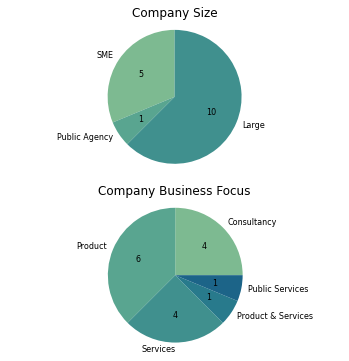
\includegraphics[width=0.5\textwidth]{images/company_views_vertical.png}
%    \caption{Descriptive data about companies involved in the study}
% \label{fig:company_data}
%\end{figure}


